\documentclass[12pt,a4paper,twoside]{book}


\usepackage[utf8]{inputenc}
\usepackage[a4paper,inner=3.5cm,outer=2.5cm]{geometry}

\usepackage[titletoc,title,toc,page]{appendix}
\usepackage{verbatim}
\usepackage{placeins}
\usepackage{listings}
\usepackage{hyperref}
\usepackage[italian]{babel}
\usepackage{tikz}
\usepackage{parskip}

\usepackage{graphicx}
\usepackage{blindtext}
\usepackage{chngcntr}
\counterwithin{table}{chapter}

\usepackage{newlfont}
\usepackage{fancyhdr}
\usepackage{indentfirst}
\usepackage[utf8]{inputenc}
\usepackage{float}
\usepackage{hyperref}
\usepackage[capitalize,noabbrev]{cleveref}
\usepackage{soul}
\usepackage[font=footnotesize,labelfont=bf]{caption}

\usepackage{multirow}
\usepackage{hyphenat}
\hyphenation{mate-mati-ca recu-perare}

\usepackage{lscape} 

\usepackage{natbib}
\bibliographystyle{alpha}
\setcitestyle{super,open={[},close={]}}

\newcommand{\rom}[1]{\uppercase\expandafter{\romannumeral #1\relax}}

\usepackage{pdfpages}

\begin{document}
% Per spostare i vari elementi più su o più giù gioca con i valori di vspace che ci sono tra uno e l'altro
\pagestyle{empty}
\newgeometry{left=2cm, right=2cm}
\begin{titlepage}
\begin{center}
    {{\Large{\textsc{Alma Mater Studiorum $\cdot$ Università di Bologna}}}}
    \rule[0.1cm]{\textwidth}{0.1mm}
    \rule[0.5cm]{\textwidth}{0.6mm}\\
    {\small{\bf SCUOLA DI SCIENZE\\
    Corso di Laurea in Informatica per il Management}}
\end{center}

\vspace{25mm}

\begin{center}
    {\LARGE{\bf ANALISI COMPARATIVA }}\\
    \vspace{3mm}
    {\LARGE{\bf DI SOLUZIONI SERVERLESS}}\\
\end{center}

\vspace{60mm}
\par
\noindent
\begin{minipage}[t]{0.04\textwidth}
~
\end{minipage}
\begin{minipage}[t]{0.4\textwidth}
{\large{\bf Relatore:\\
Chiar.mo Prof.\\
Rossi Davide}}
\end{minipage}
\hfill
\begin{minipage}[t]{0.4\textwidth}\raggedleft
{\large{\bf Presentata da:\\
De Rosa Davide}}
\end{minipage}
\begin{minipage}[t]{0.04\textwidth}
~
\end{minipage}

\vspace{30mm}

\begin{center}
    {\large{\bf \rom{2} Sessione\\
    Anno Accademico 2023/2024 }}
\end{center}
\end{titlepage}

\restoregeometry
\newpage
\begin{center}
    (DA FARE ALLA FINE)\\
    5 parole chiave per caratterizzare il contenuto della dissertazione:\\ (se non ti piacciono così sparse puoi anche semplicamente scriverle su una riga sola)
\end{center}

% https://tex.stackexchange.com/questions/26538/words-scattered-randomly-in-on-coverpage
\begin{tikzpicture}[overlay,remember picture,shift=(current page.center)]
\pgfmathsetseed{3}


\foreach [count=\count] \word in {Parola 1, parola 2, parola 3, parola 4, parola 5} {
\node [
    xshift={(mod(\count,3)-1)*(\paperwidth/4)},
    yshift={(mod(\count,7)-3)*(\paperwidth/6)},
    xshift=rand*4cm,
    yshift=rand*2cm,
    % rotate=rand*35,
    % opacity=rnd*0.5+0.125,
    font=\large] {\word};
}
\end{tikzpicture}
\newpage

\topmargin=6.5cm
\begin{flushright}
\emph{
\LARGE{La dedica}\\\vspace{2mm}
\LARGE{anche quella se vuoi}\\\vspace{3mm} 
\LARGE{su più righe} 
}
\end{flushright}
\newpage~\newpage
\pagenumbering{gobble}
\chapter*{Abstract}
Abstract qui (ti consiglio di farlo alla fine)

\topmargin=-1cm
\tableofcontents
\thispagestyle{empty}
\listoftables
\thispagestyle{empty}
\listoffigures
\thispagestyle{empty}
\newpage~\newpage


\pagenumbering{arabic}
\setcounter{chapter}{-1}
\raggedbottom
\chapter{INTRODUZIONE} \label{chap:intro}
\pagestyle{plain}
\setcounter{page}{1}

(Io l'introduzione l'ho scritta alla fine)\\
bla bla bla
\section{elenchi}
\subsection{Elenchi puntati}
\begin{itemize}
    \item bla
    \begin{itemize}
        \item sub-bla
    \end{itemize}
    \item bla
\end{itemize}

\subsection{Elenchi numerati}
\begin{enumerate}
    \item bla1
    \begin{enumerate}
        \item sub bla 1
        \item sub bla 2
    \end{enumerate}
    \item bla 2
\end{enumerate}

\subsection{Mix}
\begin{itemize}
    \item bla
    \begin{enumerate}
        \item sub bla 1
    \end{enumerate}
    \item bla
\end{itemize}

\begin{enumerate}
    \item bla 1
    \begin{itemize}
        \item sub bla
    \end{itemize}
    \item bla 2
\end{enumerate}

\section{Font}
\textbf{bla bla bla}\\
\textit{Ancora bla bla bla}\\
\texttt{bla bla ma in un'altra riga}

\subsection{Sottosezione 1 - parskip}
Grazie al package parskip se vai a capo nel .tex lasciando una riga

ti mette un po' di spazio anche nel pdf.\\
Attenzione però che ogni tanto questa feature fa lasciare troppo spazio tra testo e immagini / tabelle, se capita prova a togliere un po' di righe vuote. \\
Senza questo pacchetto, una doppia new line (\texttt{$\backslash n\backslash n$}) crea un nuovo paragrafo, la cui prima riga viene leggermente indentata (un comportamento indesiderato se vieni da altri strumenti di stesura). Eventualmente, si può usare per allungare di qualche pagina alla tesi, evitando di abusarne.
\subsection{Sottosezione 2 - capitoli}
I capitoli iniziano sempre in una pagina dispari, quindi a volte vedrai delle pagine bianche tra uno e l'altro
\subsubsection{Sottosottosezione 1} \label{subsub:bla}
bla bla bla

\chapter{Dopo l'introduzione}
qua scrivi qualcosa
\section{Immagini}
Quando fai begin figure, ricordati di mettere tra quadre un modificatore di posizione: H significa esattamente nel punto dove si trova l'immagine nel file .tex e ti consiglio di usare quello, se no ci sono ad esempio t (top) e b (bottom).

\begin{figure}[H]
    \centering
    % Se metti solo una delle due dimensioni, l'altra scala in automatico
    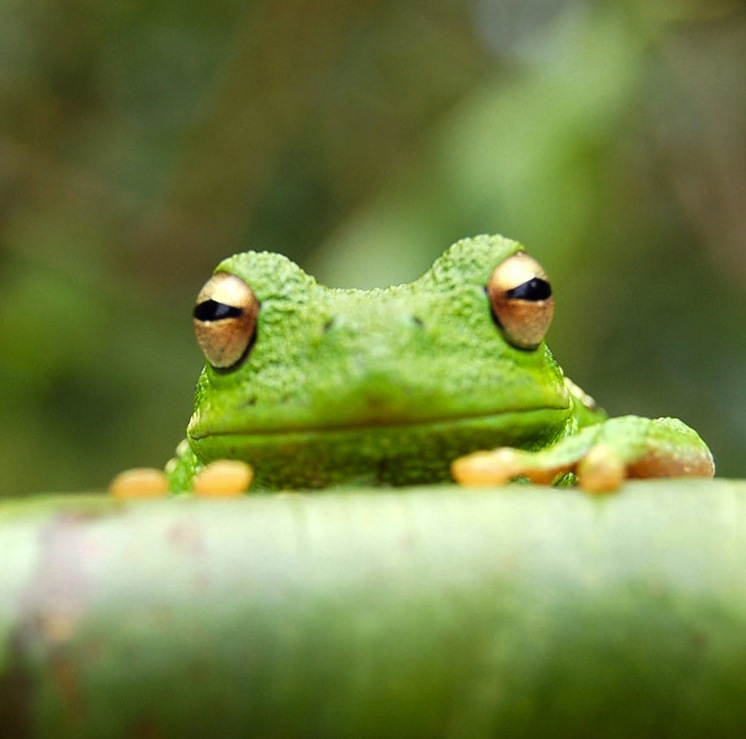
\includegraphics[height = 6cm, width=8cm]{img/frog.jpg}
    \caption{Caption (questo viene scritto nell'indice delle figure)}
    % La label ci vuole sempre e te la inventi tu: serve per riferirsi alle immagini successivamente
    \label{fig:frog}
\end{figure}

\section{tabelle}
\subsection{Tabella semplice}
Anche qui nota H tra quadre, la caption e la label

\begin{table}[H]
    \centering
    \begin{tabular}{|c|c|}
    \hline
        \textbf{Pratiche agili} & \textbf{Studenti}  \\ \hline
        Sprint planning & 73  \\ \hline
        Pair programming & 73  \\ \hline
        Retrospettiva & 48  \\ \hline
    \end{tabular}
    \caption{Tabella semplice (anche questo scritto nell'indice delle tabelle)}
    \label{tab:simple}
\end{table}

\subsection{tabelle avanzate}
Con multirow (e multicolumn che però serve meno) puoi fare righe (colonne) più grandi del normale.\\
\begin{table}[H]
    \centering
    \begin{tabular}{|c|c|c|c|c|}
    \hline
        \textbf{Team} & \textbf{LoC verificate} & \textbf{LoC sviluppatori} & \textbf{Ore sviluppatori} & \textbf{LoC/h}  \\ \hline
        \multirow{2}*{1} & 1148& m: 888& m: 40& 22\cr & Diff: -1852& $\sigma$: 371& $\sigma$: 27& \\ \hline
        \multirow{2}*{2}&1858& m: 1404& m: 65& 22\cr &  Diff: -448& $\sigma$: 1222& $\sigma$: 78& \\ \hline
        \multirow{2}*{3}&1640& m: 1400& m: 96& 15\cr &  Diff: -2810& $\sigma$: 1417& $\sigma$: 41& \\ \hline
    \end{tabular}
    \caption{CAPTION}
    \label{tab:avanz}
\end{table}

\subsubsection{Tabelle girate}
Se usi landscape la tabella viene girata (nel caso dovessi inserirne una molto grande)
\begin{landscape}
\begin{table}[H]
    \centering
    \begin{tabular}{|c|c|}
    \hline
        \textbf{Numero} & \textbf{\#}  \\ \hline
        UNO & 1  \\ \hline
        DUE & 2  \\ \hline
        TRE & 3  \\ \hline
    \end{tabular}
    \caption{Tabella girata}
    \label{tab:girata}
\end{table}

\end{landscape}

\section{Grafici}
Puoi creare grafici con tikzpicture.
Qui c'e' un grafico con asse x e y customizzabili per ogni tipo d'utilizzo.
Tutti i tool e tutorial necessari per creare ogni tipo di grafico puo' essere trovato qui: https://tikz.dev/

\begin{tikzpicture}
  % Draw x-axis
  \draw[->] (-1,0) -- (15,0) node[right] {$x$};
  % Draw y-axis
  \draw[->] (0,-1) -- (0,5) node[above] {$y$};
  
  % Draw grid lines (optional)
  \foreach \x in {1,2,3,4,5,6,7,8,9,10,11,12,13,14}
    \draw (\x,-0.1) -- (\x,0.1);
  \foreach \y in {1,2,3,4}
    \draw (-0.1,\y) -- (0.1,\y);
  
  % Draw origin
  \fill (0,0) circle[radius=2pt];
\end{tikzpicture}

\section{Import di file TeX}
Puoi importare altri file tex per intero includendoli cosi'.
Questo e' molto utile per mettere insieme diversi capitoli di una tesi o di un grande documento in generale.

Questo e' il contenuto del documento imported\textunderscore document.tex


\chapter{Altri comandi}
bla bla
\section{Math mode}
Per inserire simboli matematici (e lettere greche) serve la math mode:

Usando il simbolo del dollaro hai la math mode inline: $5 \times \alpha = 3\lambda$

Altrimenti hai quella con le barre e le quadre \[ \frac{\sum_6^i 3i\theta}{12k^2\times 7}\]

Infine hai quelle con begin equation (che vengono numerate):
\begin{equation}
    \frac{1}{2}\times A_{bcd}\times E^{fgh}
\end{equation}

Anche le equazioni possono avere label.
\section{url e footnote}
per mettere un link usa url: \url{wikipedia.it}

per fare note a piè di pagina usa footnote\footnote{Tipo questa}

\section{Code snippets}
per inserire code snippets, puoi usare lstlisting

\begin{lstlisting}[language=c]
#include<stdio.h>

int main(void) {
    printf("Hello World\n");
    return 0;
}
\end{lstlisting}

\section{verbatim}
Se ti serve scrivere codice o qualcosa per cui ti serve una formattazione specifica usa verbatim:
\begin{verbatim}
    Qui puoi scrivere

    come      vuoi
    e viene tutto

scritto
                    monospaziato
\end{verbatim}
\section{riferimenti}
Come detto prima le label servono per riferirsi ad altre parti del testo citate precendentemente.\\
Ti consiglio di metterle sempre almeno a figure. immagini e capitoli.

Per riferirti a qualcosa basta fare ref seguito dal nome della label, ad esempio ``vedi capitolo \ref{chap:intro}''.\\In questo modo dal pdf cliccando sulla reference, ti porta direttamente al punto giusto.
Altri pacchetti come \texttt{fancyref} e \texttt{cleveref} (consigliato) possono aiutare nell'automatizzare la creazione delle refrence. Usando ad esempio \texttt{\cref{chap:intro}} viene generata la dicitura corrispondete all'elemento a cui si fa riferimento, seguita dalla numerazione. Eccone un esempio: \cref{chap:intro}.
\section{citazioni}
Per citare si usa cite seguito dal nome dell'articolo nel file.bib, ad esempio ``come visto nell'articolo di tizio\cite{greenwade93}''.

Se non ti piace lo stile di citazione puoi modificarlo sopra dove scrivo usepackage natbib, ma quello impostato attualmente dovrebbe andare bene.



\renewcommand{\bibsection}{}
\chapter*{Riferimenti bibliografici}
\bibliography{refs}
\newpage

\renewcommand{\appendixtocname}{Appendici}
\renewcommand{\appendixpagename}{Appendici}
% \csname @openrightfalse\endcsname
\pagenumbering{gobble}
\begin{appendices}
\chapter{Appendice 1}
\label{Appendice:A}
Probabilmente ci sono un sacco di package non utilizzati ma così funziona tutto quindi non ho indagato oltre.

Inoltre su internet c'è un sacco di documentazione se ti servisse.
\chapter{Appendice B}
\label{Appendice:B}
Appendice B se serve

\chapter{Embed di interi PDF}
\label{Appendice:C}
Se ti serve puoi fare embed di PDF interi con pdfpage, scegliendo anche le pagine (o mettendo - se le vuoi tutte):

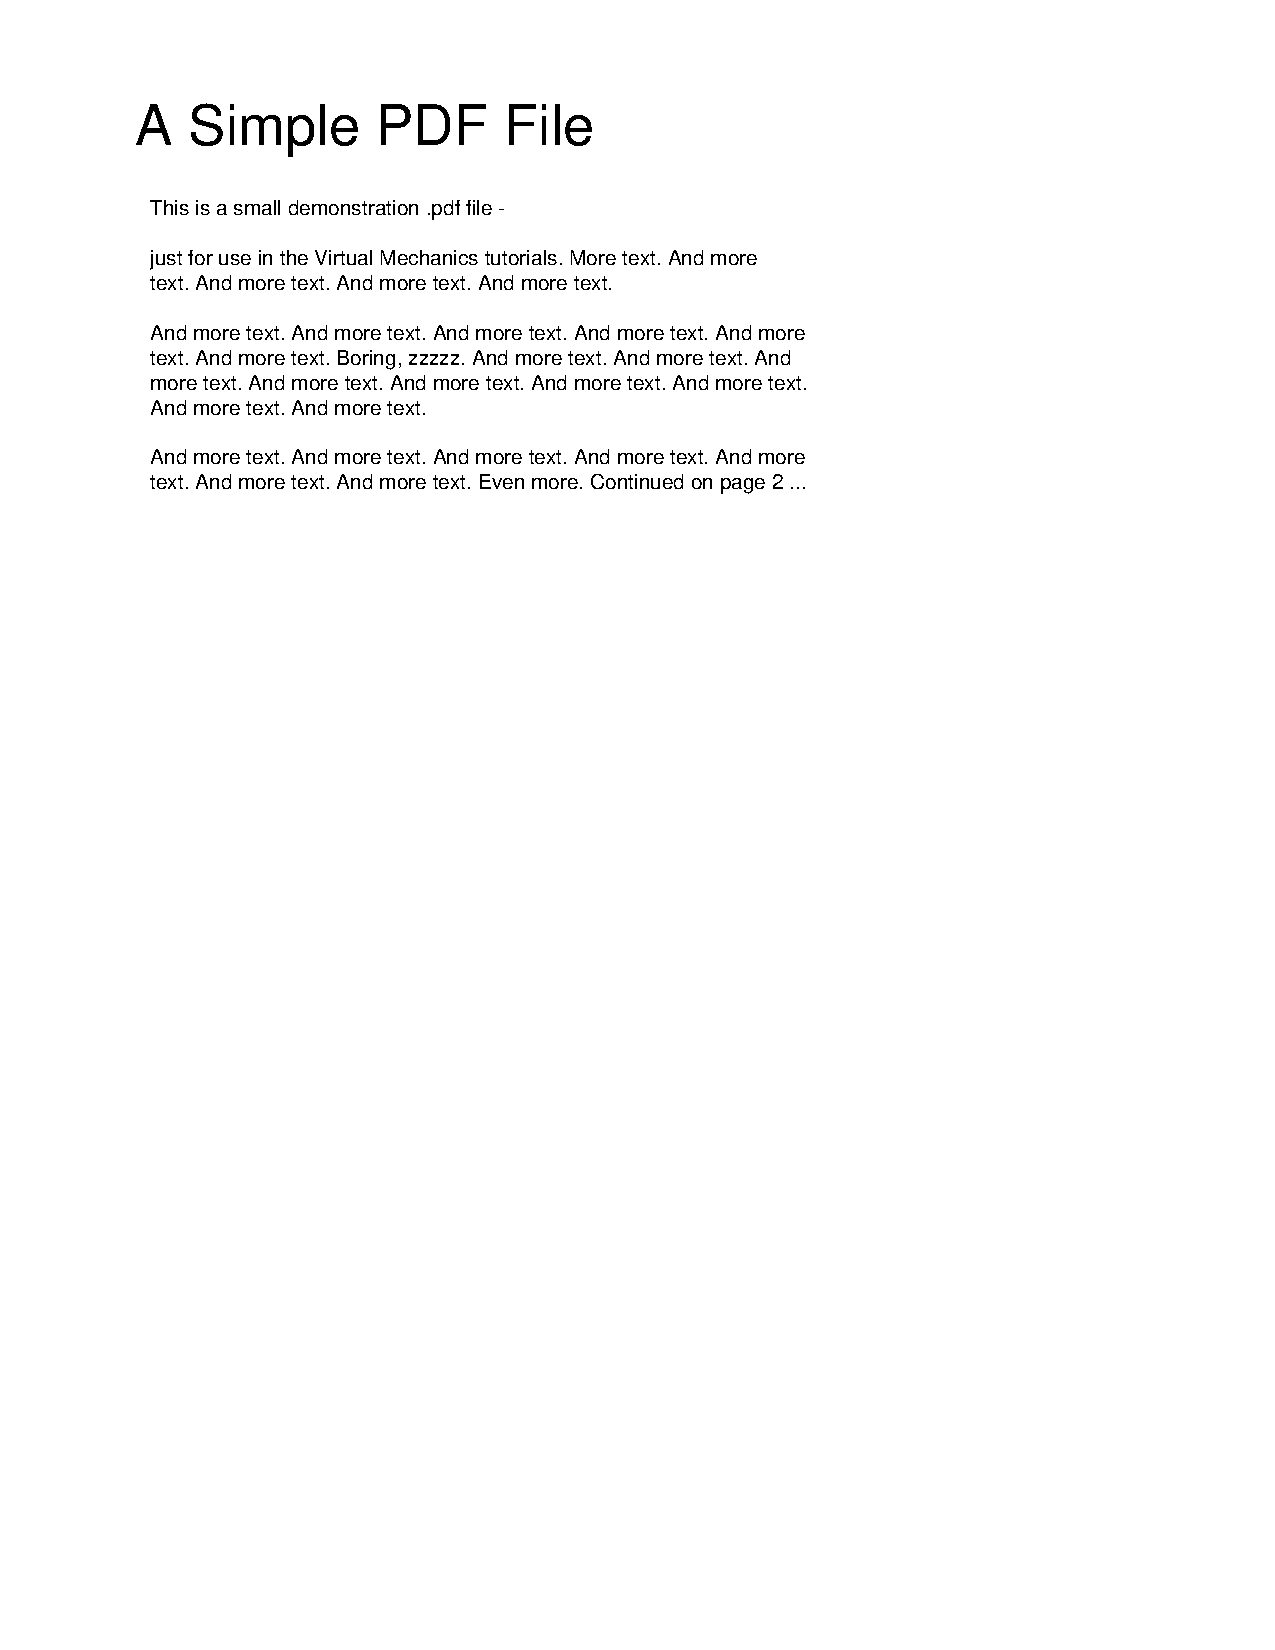
\includepdf[pages=1]{pdf/sample.pdf}
\end{appendices}

\newpage~\newpage
\chapter*{Ringraziamenti}
Grazie a tutti
\end{document}